% 2007 年新课标卷文科第 18 题：空间四点 A、B、C、D，△ADB 以 AB 为轴转动。
%   D 为顶点，A、B 为轴的两端，C 为底面点；AB 被面 DBC 遮挡，画虚线。
% 来源 PDF：gaokaomath-src/普通高考/2007/2007新课标文(海南,宁夏).pdf
% SHA-256：920ab7ed3244ae8c738e34446fd4135b3a5c50c71fb5e03c3eba0f8a7cbcf804
% 原页：2007新课标文(海南,宁夏).pdf 第 1 页（A3 三栏）第 3 栏，书页码 395。
% 重绘依据：按原页 D、A、B、C 的相对位置与虚实线重绘。
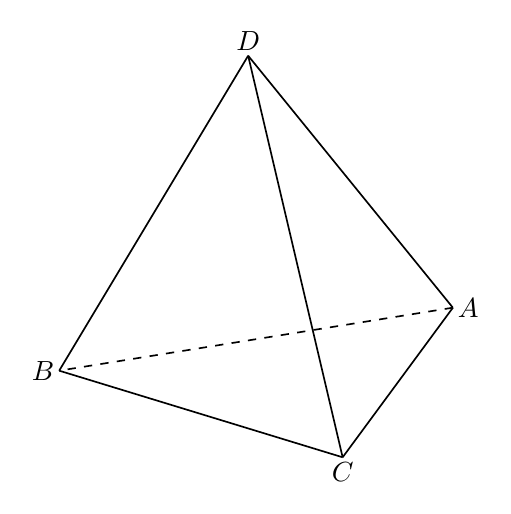
\begin{tikzpicture}[scale=1.0, semithick,
  every node/.style={inner sep=1.5pt}]

  \coordinate (D) at (0,4.0);
  \coordinate (A) at (2.6,0.8);
  \coordinate (B) at (-2.4,0.0);
  \coordinate (C) at (1.2,-1.1);

  \draw (D) -- (A);
  \draw (D) -- (B);
  \draw (D) -- (C);
  \draw (A) -- (C);
  \draw (B) -- (C);
  \draw[dashed] (A) -- (B);

  \node[above] at (D) {$D$};
  \node[right] at (A) {$A$};
  \node[left] at (B) {$B$};
  \node[below] at (C) {$C$};
\end{tikzpicture}
